\documentclass[twoside,leqno,11pt]{article}
\usepackage{revstat-v2}
\usepackage{amsmath}
\usepackage{enumerate}
\usepackage{amssymb}
\usepackage{graphicx}
\usepackage{hyperref}
\usepackage{color}
\usepackage[utf8]{inputenc}
\usepackage[T1]{fontenc}
\usepackage{pdflscape}
\usepackage{bm}
\usepackage{float}
\usepackage{listings}
\usepackage{xcolor}
\usepackage{color}
\usepackage{caption}
\usepackage{subcaption}

\usepackage{hyperref}
\hypersetup{
	pdftoolbar=true,        % show Acrobat’s toolbar?
	pdfmenubar=true,        % show Acrobat’s menu?
	pdffitwindow=true,     % window fit to page when opened
	pdfstartview={FitH},    % fits the width of the page to the window
	pdftitle={title},    % title
	pdfauthor={Salvatore Mazzarino},     % author
	pdfsubject={Subject},   % subject of the document
	pdfcreator={Salvatore Mazzarino},   % creator of the document
	pdfproducer={Salvatore Mazzarino}, % producer of the document
	pdfkeywords={Green Networking} {Mobile Cloud} {Network Coding} {Energy}, % list of keywords
	pdfnewwindow=true,      % links in new window
	colorlinks=true,       % false: boxed links; true: colored links
	linkcolor=blue,          % color of internal links (change box color with linkbordercolor)
	citecolor=blue,        % color of links to bibliography
	filecolor=magenta,      % color of file links
	urlcolor=magenta           % color of external links
}
\newcommand{\etn}{{\mbox{\boldmath $\eta$}}} 
\hyphenation{ge-ne-ra-ted  hy-per-geo-me-tric  cha-rac-te-ri-ze}
 
\begin{document}
\thispagestyle{firstpage}

\vspace{-3.2cm}

\noindent
{\footnotesize {\sffamily REVSTAT~~--~~Statistical~~Journal\\[-1pt]
		Volume 0, Number 0, Month 0000,
		000-000}}
% \thepage-\pageref{LastPage}}}   % requires \usepackage{lastpage}

\vspace{1.5cm}
\title{The Marshall and Olkin-G and Gamma-G family of distributions: properties and applications}

\renewcommand{\titleheading}
{The MOGG family of distributions}  % --- on odd running heads

\author{\authoraddress{Maria do Carmo S. Lima \href{https://orcid.org/0000-0002-5480-3103}{
\includegraphics[scale=0.08]{ORCID-iD_icon-128x128}}} 
	{Department of Statistics,
		Federal University of Pernambuco,\\
        Pernambuco, Recife, Brazil
        \href{maria@de.ufpe.br}{maria@de.ufpe.br}}
	\\
	\authoraddress{Gauss M. Cordeiro \href{https://orcid.org/0000-0002-3052-6551}{
\includegraphics[scale=0.08]{ORCID-iD_icon-128x128}}}
	{Department of Statistics,
		Federal University of Pernambuco,\\
		Pernambuco, Recife, Brazil
		\href{gauss@de.ufpe.br}{gauss@de.ufpe.br}}
	\\
	\authoraddress{Pedro Rafael D. Marinho \href{https://orcid.org/0000-0003-1591-8300}{
\includegraphics[scale=0.08]{ORCID-iD_icon-128x128}}
	\correspondingauthor}
	{Department of Statistics,
		Federal University of Paraíba,\\
		Paraíba, João Pessoa, Brazil
		\href{pedro.rafael.marinho@gmail.com}{pedro.rafael.marinho@gmail.com}}
}
\renewcommand{\authorheading}
{Maria do Carmo S. Lima, Gauss M. Cordeiro and Pedro Rafael D. Marinho, }  % --- on even running heads

%\vspace{0.3in}
%First Version: 27 July 2010\\
%\vspace{0.1in}
%This Version: 27 January 2011\\

%-------------------------------------------------------------------------------
% Just asking LaTeX to effectively do the title...
%-------------------------------------------------------------------------------
\maketitle
%-------------------------------------------------------------------------------
% Just asking LaTeX to numerate lines...
%-------------------------------------------------------------------------------
\setpagewiselinenumbers
\modulolinenumbers[1]
%\linenumbers
%%%%%%%%%%%%%%%%%%%%%%%%%% alteracao: Datas %%%%%%%%%%%%%%%%%%%%%%%%%%%%%%%%%%
\noindent
~~~~{\small{\sffamily Received:} December 2020 ~~~~~~{\sffamily Revised:} May 2022 ~~~~~~{\sffamily Accepted:} Month 0000}
%%%%%%%%%%%%%%%%%%%%%%%%%% alteracao %%%%%%%%%%%%%%%%%%%%%%%%%%%%%%%%%%

%-------------------------------------------------------------------------------
% Abstract of the article...
%-------------------------------------------------------------------------------
\begin{abstract}
The article introduces a new family by combining the Marshall and Olkin-G and Gamma-G classes. It has only two
extra shape parameters and can be a better model than other existing classes of distributions. Simulations are performed to verify the consistency of the estimators. Its flexibility is shown by means of two real data sets.
\end{abstract}

%-------------------------------------------------------------------------------
% Keywords...
%-------------------------------------------------------------------------------
\begin{keywords}
Applications; distribution family; mathematical properties; simulations. 
\end{keywords}

%-------------------------------------------------------------------------------
% AMS classifications...
%-------------------------------------------------------------------------------
\begin{ams}
60E05, 62E10, 62E15.
\end{ams}

\section{INTRODUCTION}

The advances in the field of Data Science requires the search for new fa\-milies of distributions that adequately model real data has been increasing steadily in the last years.  The construction of different generation methods and even generators of families has made it difficult to compare new proposals. In the midst of a huge set of existing families in the literature of new distributions, to find a proposal that is in fact an excellent competitor when compared to other existing ones, in terms of adjustment to real data sets and also that does not present estimation problems, is a major challenge.

The classes of distributions in the early 1980s were based on the simple idea of adding parameters to a baseline distribution. The mechanism by adding shape parameters to a baseline distribution has proved to be useful to make the 
generated distributions more flexible especially for studying  tail properties than existing ones and for improving their goodness-of-fit statistics to real data. Many special  distributions in these families are discussed by Tahir and Nadarajah (2015) \cite{Tahir}.

The addition of parameters in the construction of new distributions/families was improved by the inclusion of mathematical functions known in the literature, such as beta and gamma functions, for example, which produce new generators with more flexible properties than their baselines. Two well-known examples are the beta-G (Eugene et al., 2002)  \cite{Eugene} and gamma-G (Zografos and Balakrishnan, 2009) \cite{Zografos} generators.

However, the inclusion of such functions for generating new families brought, in some cases, problems for parameter estimation. So, despite the fit being more suitable for some types of data and, therefore, having a superior performance when compared to other generators, the estimation process can  often be a problem.

In this context, this work presents a new family obtained by composing a very competitive class in the literature with another class that has the gamma function in its structure.

Let $G(x)$ be the cumulative distribution function (CDF) of a baseline distribution and $g(x)=dG(x)/dx$ be the corresponding  probability density function (PDF) depending on a parameter vector $\eta$. A generalized family is presented with two extra shape parameters by transforming the CDF $G(x)$ according to two sequential important classes.  These classes, called Marshall and Olkin-G and Gamma-G, are important for modeling data in several areas,  and they are reviewed below. 


The CDF of the Marshall and Olkin's (1997) \cite{Marshall} ($\text{MO-G}$) 
class (for $\theta>0$) is
\begin{equation}\label{CDF_MO}
F_{\text{MO-G}}(x)=\frac{G(x)}{\theta+(1-\theta)G(x)}=\frac{G(x)}{1-(1-\theta)[1-G(x)]},\quad x \in \mathbb{R}.
\end{equation}

The density function corresponding to (\ref{CDF_MO}) has the form
\begin{equation}\label{densityMO}
f_{\text{MO-G}}(x)=\frac{\theta\, g(x)}{[\theta+(1-\theta)G(x)]^{2}}.
\end{equation}

For $\theta=1$, $f_{\text{MO-G}}(x)$ is equal to $g(x)$. 
Equation \eqref{densityMO} represents the PDF of the minimum of $n$ iid random variables having density $g(x)$, say $T_1,\cdots,T_N$, 
where $N$ has a geometric distribution with probability parameters $\theta$ and $\theta^{-1}$ if $0<\theta<1$ and $\theta>1$, 
respectively.

Tahir and Nadarajah (2015, Table 2) \cite{Tahir} presented thirty  distributions belonging to this family. It is easily generated  from the baseline quantile function (QF) by $Q_{\text{MO-G}}(u)=Q_{G}\left(\theta u / \left[\theta u+1-u\right]\right)$ for $u\in(0,1)$.

Marshall and Olkin considered the exponential and Weibull distributions for the baseline G and derived some
structural properties of the generated distributions. 
If G is an exponential distribution, the special case 
refers to a two-parameter competitive model to the 
Weibull and gamma distributions.

The CDF of the gamma-G ($\Gamma$-G) class (Zografos and Balakrishnan, 2009) \cite{Zografos}  is
\begin{eqnarray}\label{CDF_Ga}
F_{\Gamma\text{-G}}(x)=\gamma_1\left( a, -\log \left[1-G(x)\right]\right), \quad x \in \mathbb{R},
\end{eqnarray}
where $a>0$ is an extra shape parameter, $\gamma_1(a,z)= \gamma(a,z)/\Gamma(a)$ is the incomplete gamma function ratio, 
and $\gamma(a,z)=\int_0^{z} t^{a-1}\,\rm{e}^{-t}dt$.

Then, the PDF of the $\Gamma$-G class can be expressed as
\begin{eqnarray}\label{PDF_Ga}
\displaystyle
f_{\Gamma\text{-G}}(x)=\frac{\displaystyle 1}{\displaystyle \Gamma(a)} \left\{ -\log[1-G(x)] \right\}^{a-1}\, g(x).
\end{eqnarray}

Each new $\Gamma$-G distribution follows from a given 
baseline G. For $a=1$, the $\Gamma$-G class reduces to G.
If $Z$ is a gamma random variable with unit scale
and shape $a>0$, then $W=Q_G(1-\rm{e}^{-Z})$ has density (\ref{PDF_Ga}). So, the $\Gamma$-G distribution is easily 
generated from the gamma distribution and the QF of G.

The remaining of the paper is addressed as follows. Section \ref{sec:MOGaG} introduces the {\it Marshall and Olkin-Gamma-G} (MOGa-G) family, and provides some special models. The maximum likelihood estimates (MLEs) of its parameters is addressed in Section \ref{estimation}. Some simulations are performed in Section \ref{sec:simulation} to estimate the biases of the MLEs. Two empirical applications illustrate the potentiality of the proposed family in Section \ref{applications}. A variety of theoretical properties are obtained in Section \ref{properties}. Some conclusions remarks are offered in Section \ref{conclusions}.

\section{THE NEW FAMILY}\label{sec:MOGaG}

By combining Equations (\ref{CDF_MO}) and (\ref{CDF_Ga}), the CDF of the random variable $X\sim$MOGa-G representing the new family 
has the form 
\begin{equation}\label{CDF_MO-Gamma-G}
F_{X}(x)=\frac{\gamma_1\left( a, -\log \left[1-G(x)\right]\right)}{\theta+(1-\theta)\gamma_1\left( a, -\log \left[1-G(x)\right]\right)},\quad x \in \mathbb{R}.
\end{equation}

By differentiating (\ref{CDF_MO-Gamma-G}), the PDF of $X$ follows as
\begin{equation}\label{PDF_MO-Gamma-G}
f_{X}(x)=\frac{\theta  \left\{ -\log[1-G(x)] \right\}^{a-1}\, g(x)}{\Gamma(a)\,\left\{\theta+(1-\theta)\gamma_1\left( a, -\log \left[1-G(x)\right]\right)\right\}^{2}}.
\end{equation}

The density (\ref{PDF_MO-Gamma-G}) can be interpreted from a sequence of $N$ iid random variables, say $Z_1,\cdots,Z_N$,
each one having a gamma density with unit scale and shape $a>0$, assuming that $N$ (is not fixed) has a geometric 
distribution with probabilities $\theta$ and $\theta^{-1}$ for $0<\theta<1$ and $\theta>1$,
respectively. By transforming the $Z_i$'s via the baseline QF by $W_i=Q_G(1-\rm{e}^{-Z_i})$ (for $i=1,\ldots,N$), Equation \eqref{densityMO} defines the PDF of the minimum $W_1,\cdots,W_n$. 
The proposed family from the double composition of the two 
classes absorbs the impacts of their different flexibilities on real applications. 


Table 1 provides some special cases of (\ref{PDF_MO-Gamma-G}), where $\Phi(x)$ and $\phi(x)$ are the CDF and PDF of the standard normal distribution. The density and hazard ($h(x) = f(x)/[1-F(x)]$) functions of the MOGa-Weibull (MOGa-W) model 
are displayed in Figure \ref{formas}, which provide more flexibility to both functions for both classes applied separately to the Weibull model. 

\vspace{0.6cm}

%\begin{figure}[H]
%\begin{center}
%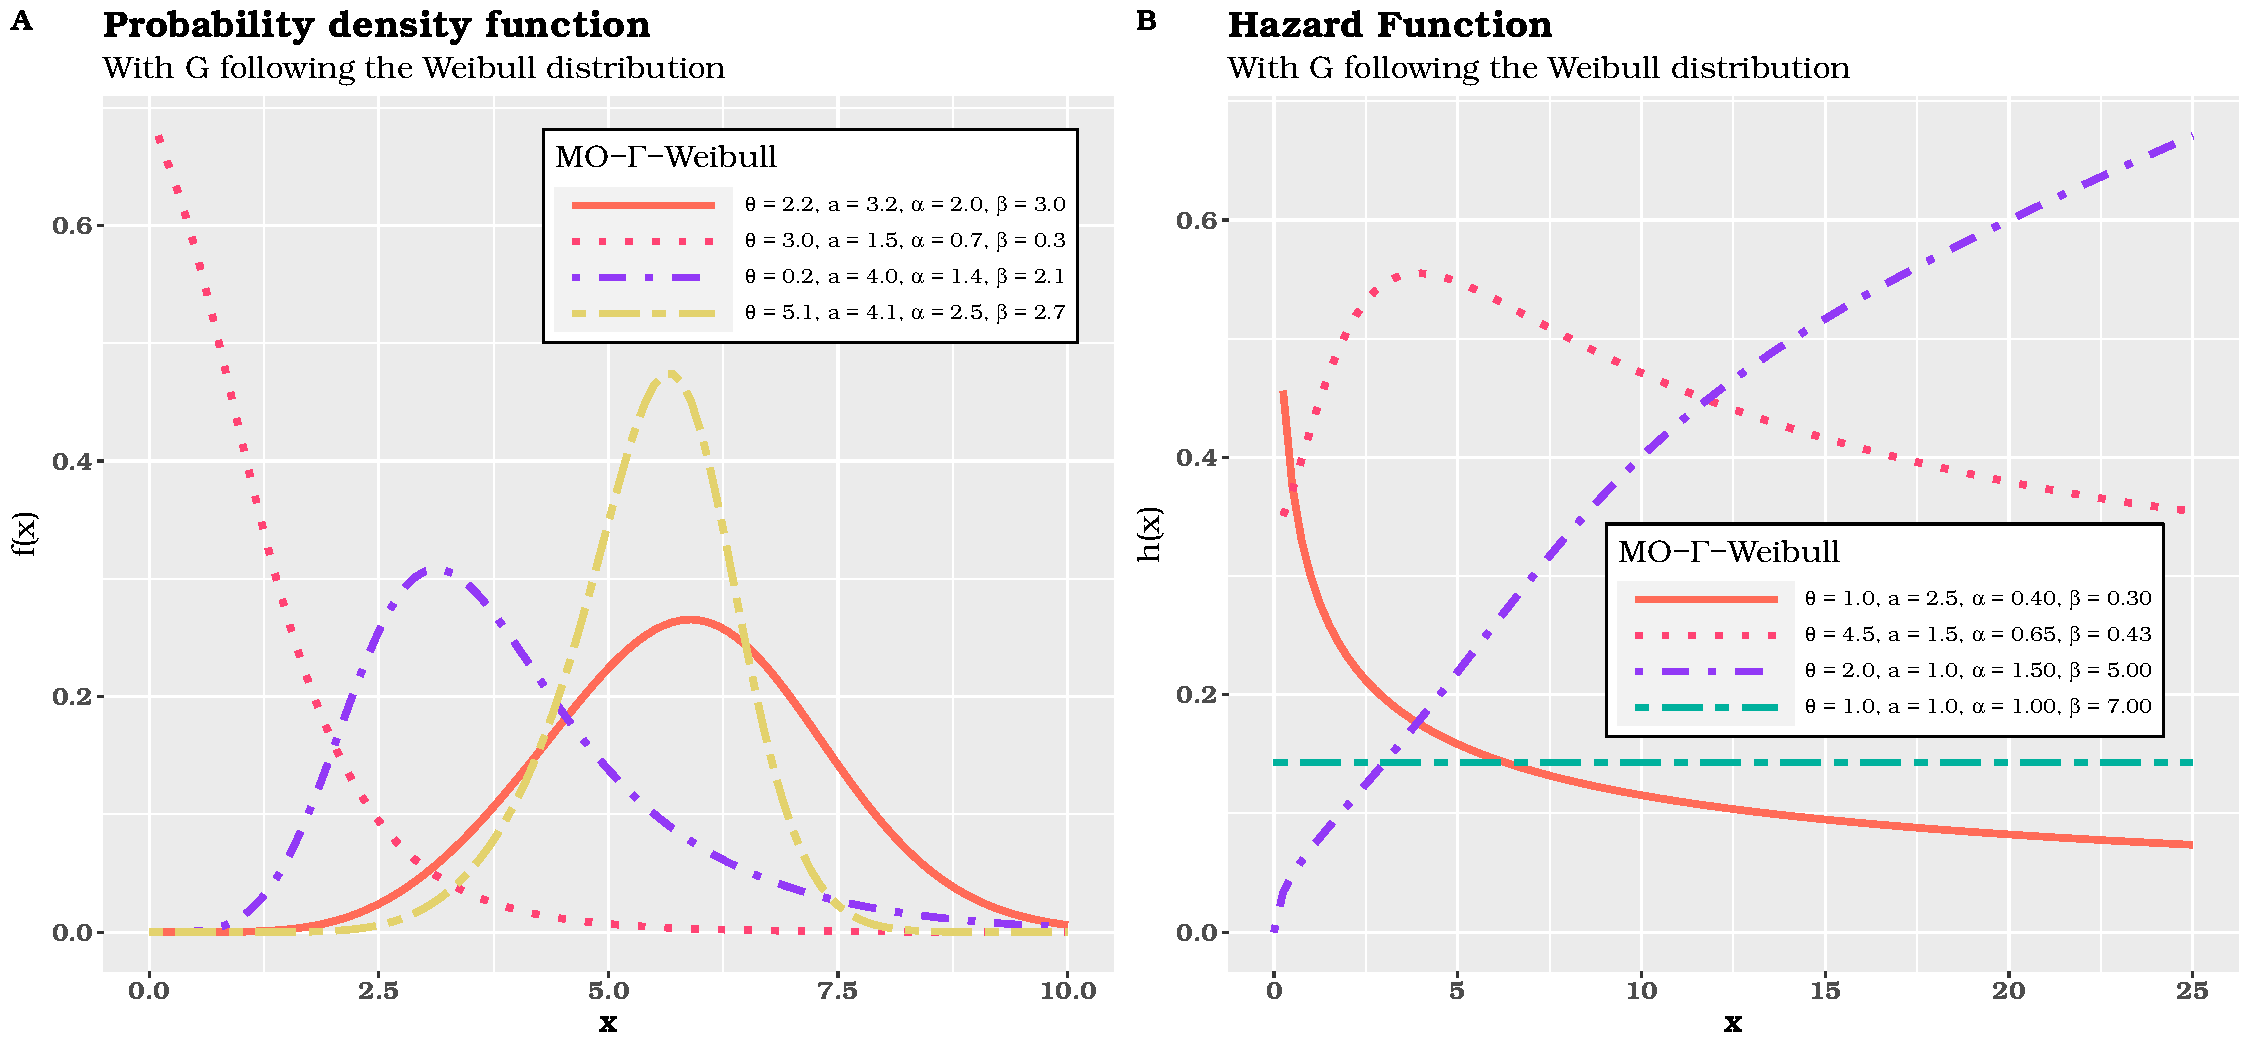
\includegraphics[scale =  0.39]{pdf-hazard.pdf}
%\caption{(A) MOGa-W density. (B) MOGa-W hazard.\label{formas}}
%\end{center}
%\end{figure}

\begin{figure}[H]
	\centering
	\begin{subfigure}[b]{0.49\textwidth}
		\centering
		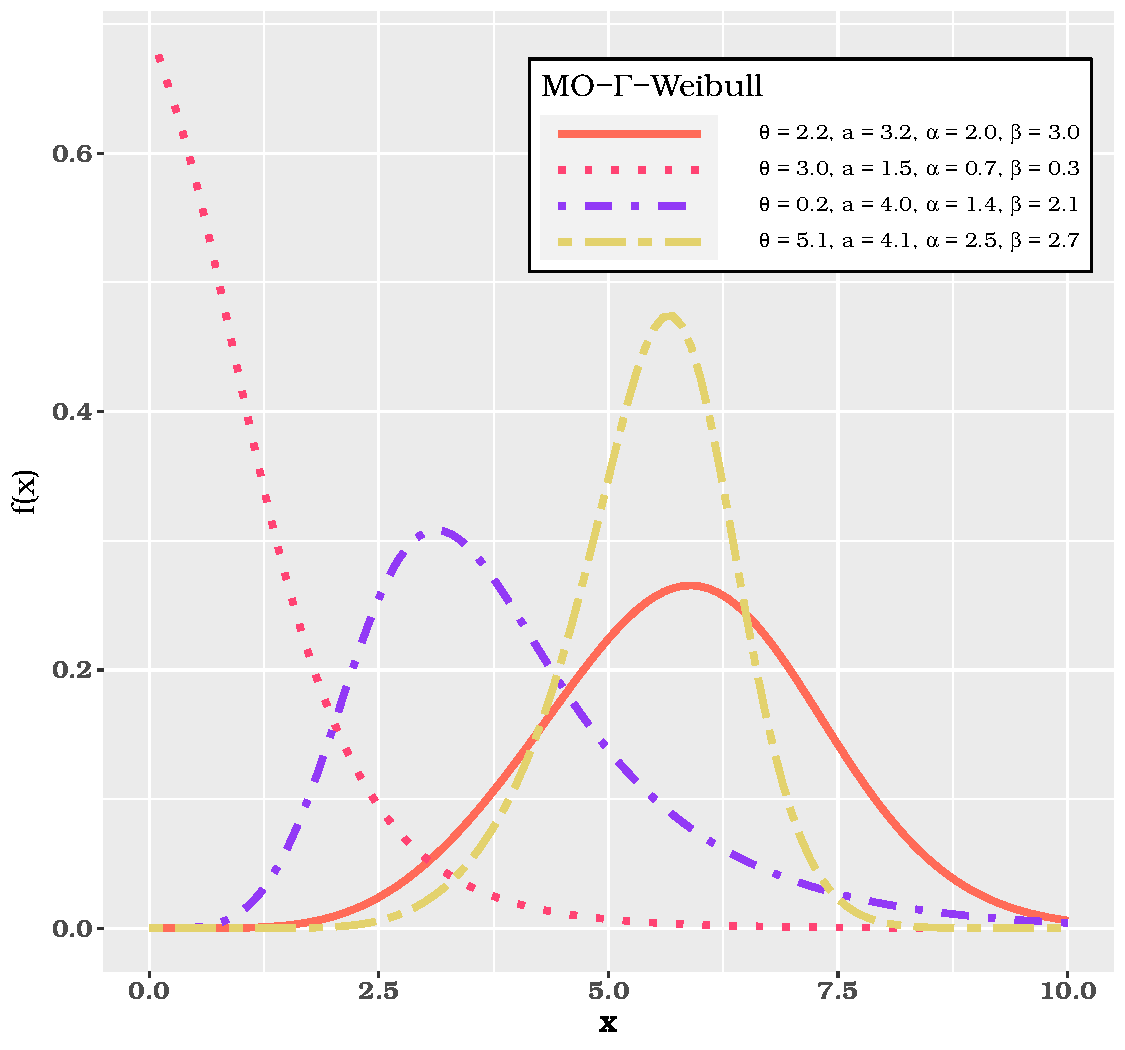
\includegraphics[width=\textwidth]{pdf_function.pdf}
		\caption{Density function.}
		\label{fig:pdf}
	\end{subfigure}
	\hfill
	\begin{subfigure}[b]{0.49\textwidth}
		\centering
		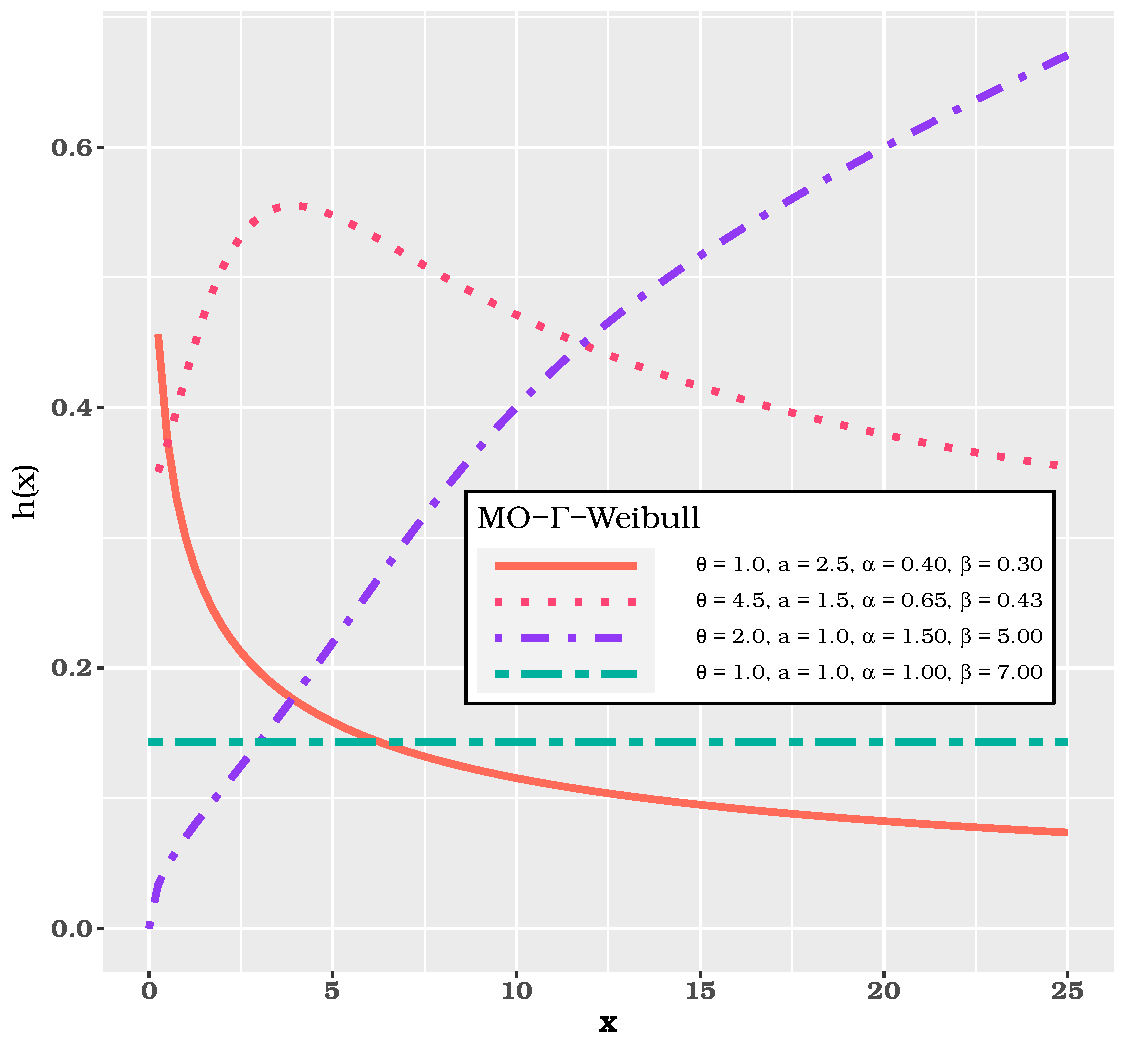
\includegraphics[width=\textwidth]{hazard_function.pdf}
		\caption{Hazard function.}
		\label{fig:hazard}
	\end{subfigure}
\caption{The density and hazard functions of the MOGa-W model.}
\label{formas}
\end{figure}

\vspace{0.6cm}

The CDF \eqref{CDF_MO-Gamma-G} can be easily inverted to 
calculate the QF of the MOGa-G distribution, say $x=Q_{X}(u)=F_X^{-1}(u)$ (for $u \in (0,1)$), in terms of 
the baseline QF $Q_G(\cdot)$. The inverse of
$F_{X}(x)=u$, where $u$ is a uniform number in $(0,1)$, 
follows by combining the inverses of Equations (\ref{CDF_MO}) and \eqref{CDF_MO-Gamma-G}. So, $F_{X}(x)=u$ gives 
$z=z(u)=\theta u/[1-(1-\theta)u]$ and $\gamma_{1}\left(a, -\log[1-G(x)]\right)=z(u)$. Hence, the QF of $X$ can be 
expressed as
$$x=Q_G\left(v(u)\right),$$
where
$$v(u)=1-\exp\left[-\gamma_1^{-1}\big(a,z(u)\big)\right],$$
and $\gamma_1^{-1}(a,w)=Q^{-1}(a,1-w)$ is the inverse function of $\gamma_1(a,w)$. Some formulae for
$Q^{-1}(a,1-w)$ are given in \url{http://functions.wolfram.com/GammaBetaErf/InverseGammaRegularized/}.

%\begin{landscape}
\begin{table}[H]\label{tabspecial1}
\caption{Special Distributions in the  MOGa-G family.}
\centering
\scalebox{0.73}{
\begin{tabular}{l|l|l}
\hline
\textbf{Distribution} & \textbf{Baseline CDF} & \textbf{Generated PDF}  \\
\hline
{} & {} & {} \\
\textbf{Normal} &  $G(x)=\Phi(x)$ & $f_{X}(x)=\frac{\theta  \left\{ -\log[1-\Phi(x)] \right\}^{a-1}\, \phi(x)}{\Gamma(a)\,\left\{\theta+(1-\theta)\gamma_1\left( a, -\log \left[1-\Phi(x)\right]\right)\right\}^{2}}$ \\
{} & {} & {} \\
\hline
{} & {} & {} \\
\textbf{Logistic} &  $G(x)=\frac{1}{1+\rm{e}^{-x}}$ & $f_{X}(x)=\frac{\theta\,\rm{e}^{-x}\, \left\{ -\log[1-(1+\rm{e}^{-x})^{-1}] \right\}^{a-1}}{\Gamma(a)\,(1+\rm{e}^{-x})^{2}\,\left\{\theta+(1-\theta)\gamma_1\left( a, -\log \left[1-(1+\rm{e}^{-x})^{-1}\right]\right)\right\}^{2}}$\\
{} & {} & {} \\
\hline
\textbf{Gumbel} &  $G(x)=1-\exp(-\rm{e}^x)$ & $f_{X}(x)=\frac{\theta \, \exp(a \,x-  \rm{e}^x)}{\Gamma(a)\,\left\{\theta+(1-\theta)\gamma_1\left(a, \rm{e}^{x}\right)\right\}^{2}}$ \\
{} & {} & {} \\
\hline
{} & {} & {} \\
\textbf{Log-Normal} &  $G(x)=\Phi(\log x)$ & $f_{X}(x)=\frac{\theta\,\phi(\log x)\,  \left\{ -\log[1-\Phi(\log x)] \right\}^{a-1}}{\Gamma(a)\,x\,\left\{\theta+(1-\theta)\gamma_1\left( a, -\log \left[1-\Phi(\log x)\right]\right)\right\}^{2}}$ \\
{} & {} & {} \\
\hline
{} & {} & {} \\
\textbf{Exponential} &  $G(x)=1-\exp(-\lambda x),\,\lambda>0$ & $f_{X}(x)=\frac{\theta\,\lambda^{a}\,x^{(a-1)}\, }{\Gamma(a)\,\left\{\theta+(1-\theta)\gamma_1\left(a,\lambda x\right)\right\}^{2}}$ \\
{} & {} & {} \\
\hline
{} & {} & {} \\
\textbf{Weibull} &  $G(x)=1-\exp(-(\lambda x)^\gamma),\,\lambda,\gamma>0$ & $f_X(x)=\frac{\theta\,\gamma\lambda^{a\,\gamma}x^{a\,\gamma-1}\exp\{-(\lambda\,\gamma)^\gamma\}}{\Gamma (a)\{\theta+(1-\theta)\gamma_1[a,(\lambda\,x)^\gamma]\}^2}$ \\
{} & {} & {} \\
\hline
{} & {} & {} \\
\textbf{Gamma} &  $G(x)=\gamma_1(\alpha,\beta x),\,\alpha,\,\beta>0$ & $f_{X}(x)=\frac{\theta\,\beta^{\alpha}\,x^{\alpha-1}\,\rm{e}^{-\beta x}\,\left\{ -\log[1-\gamma_1(\alpha,\beta x)] \right\}^{a-1}}{\Gamma(a)\,\left\{\theta+(1-\theta)\gamma_1\left( a, -\log \left[1-\gamma_1(\alpha,\beta x)\right]\right)\right\}^{2}}$ \\
{} & {} & {} \\                                                                                                                                                                          \hline
\textbf{Pareto} &  $G(x)=1-\frac{1}{(1+x)^\nu},\,\nu>0$ & $f_{X}(x)=\frac{\theta \, \rm{e}^{-x}\, \left[\nu\log(1+x)\right]^{a-1}\, g(x)}{\Gamma(a)\,(1+\rm{e}^{-x})^2\,\left\{\theta+(1-\theta)\gamma_1\left( a, \nu\log[1+x]\right)\right\}^{2}}$\\
{} & {} & {} \\
\hline
\textbf{Dagum} & $G(x) = [1 + (x/\beta) ^ {-\alpha}] ^ {-p},\,\, \alpha, \beta, p > 0$ & $f_X(x) = \frac{\theta  \left\{ -\log[1-[1 + (x/\beta) ^ {-\alpha}] ^ {-p}] \right\}^{a-1}\, g(x)}{\Gamma(a)\{\theta + (1 - \theta)\gamma_1[a, -\log   (1-((x/\beta)^{-\alpha}+1)^{-p})]\}}$ \\
\hline
\end{tabular}}
\end{table}
%\end{landscape}

\section{ESTIMATION}\label{estimation}

The MOGa-G family can be fitted to real data using the {\bf AdequacyModel} package (Marinho et al., 2019)  \cite{Marinho} in the {\sf R} software. This packa\-ge does not require to  define the log-likelihood function, and it computes the MLEs,  their standard errors (SEs), and the formal statistics defined  in Section \ref{applications}. It is only necessary to provide the PDF and CDF of the distribution to be fitted to a data set.

For example, if $x_i$ is one observation from (\ref{PDF_MO-Gamma-G}) and $\etn$ is a $q$-parameter vector specifying $G(\cdot)$ as the Weibull CDF, the log-likelihood function for $\boldsymbol{\theta}^\top=(a,\theta,\etn^\top)$ from $n$ observations can be expressed as 
\begin{align}\label{loglik}
\ell (\boldsymbol{\theta})=&\,n\log (\theta)+n\log(\gamma)+n\, a\, \gamma \log(\lambda)+(a\gamma-1)\sum_{i=1}^n{\log(x_i)}-\lambda^\gamma\sum_{i=1}^n x_i^\gamma\nonumber \\ &
-n\log[\Gamma(a)]-2\sum_{i=1}^n{\log\{\theta+(1-\theta)\gamma_1[a,(\lambda\,x_i)^\gamma]\}}.
\end{align}

Due to the impossibility of obtaining the MLEs in closed form, numerical methods to calculate the estimates that maximize $\ell(\cdot)$ are necessary. Several programming languages and statistical software provides functions and routines that make it easy to obtain numerical estimates by various interactive methods. In practice, these estimates are commonly found in this way, since the Newton and quasi-Newton methods produce satisfactory results under reasonable conditions of the object function, i.e., when they do not impose restrictions that disturb the convergence of 
the algorithms.

The {\bf AdequacyModel} package of the programming language {\sf R} is used to obtain the MLEs, see R Core Team (2020) \cite{Team}. This library, created and maintained by one of the authors of this paper,
is widely cited by several works in statistics, and serves as 
a basis for other library implementations available on the Comprehensive R Archive Network (CRAN). By using the goodness.fit function, it is possible to provide an implementation  
of (\ref {PDF_MO-Gamma-G}), and obtain $\ell(\cdot)$ by returning the MLEs, and some measures of adequacy of fit. Further details regarding this package can be obtained from Marinho et al. (2019) \cite{Marinho}.


\section{SIMULATIONS}\label{sec:simulation}

Due to the probable absence of MLEs in closed-form for distributions belonging to the MOGa-G family, it is necessary to examine the precision of the estimates calculated numerically. 

In order to do that, the biases of the estimators of the 
parameters of the MOGa-Dagum($\theta,a,\alpha,\beta,p$) and  MOGa-Weibull($\theta,a,\lambda,\gamma$) distributions 
are determined, where $G\sim \mathrm {Dagum} (\alpha,\beta,p)$ and $\mathrm {Weibull} (\gamma,\lambda)$ are the baseline models, respectively. All parameters are taken equal to 
one for different sample sizes reported in Tables \ref{tab:bias1} and \ref{tab:bias2}. 

The numbers in Tables \ref{tab:bias1} and \ref{tab:bias2} 
indicate that the estimation method behaves well when the 
sample size increases. This is theoretically expected. However, 
in practice, difficulties can be faced to other families due 
to the flatness of the log-likelihood function.

All Monte Carlo simulations can be reproduced using the script 
in \url{https://github.com/prdm0/MOGG}. The simulations are parallelized and able to use all threads available by a multicore processor, thus making them more computa\-tio\-nally efficient, 
and consequently requiring less time to complete. 

The simulations are performed on a computer with an Intel(R) Core(TM) i5-9500 CPU processor with 6 threads working at a maximum frequency of 3.00GHz, requiring, on this hardware, a time of 15.4828 hours to perform all simulations, 7.7414 hours for the MOGa-Dagum($\theta, a, \alpha, \beta, p$) distribution, 
and 4.9688 hours for the MOGa-Weibull($\theta, a, \lambda, \gamma$) distribution. Tables \ref{tab:bias1} and  \ref{tab:bias2} 
reveal that the average biases of the MLEs could be very small for $n>2,000$.

To generate observations from the random variable $X$ with density $f$, the well-known Acceptance-Rejection Algorithm for 
continuous random variables is very useful when the QF involves complex functions that can lead to some numerical inaccuracies. For doing this, another random variable $Y$ is chosen such that it can generate observations from a PDF $h$ with the same support as $f$. Then, the acceptance and rejection algorithm is defined by the following steps:
\begin{enumerate}
	\item Generate an outcome $y$ from $Y$;
	\item Generate an observation $u$ from a random variable $U\sim \mathcal{U}(0,1)$;
	\item If $u < \frac{f(y)}{c\, g(y)}$, where $c$ is a real constant, accept $x=y$; otherwise reject $y$ as an outcome from $X$ and return to 1.
\end{enumerate}

The constant $c$ must be chosen in such a way that $\frac{f(y)}{c \,g (y)}\leq 1 $. Thus, to minimize the computational cost of generating observations from $X$ through the generated observations from $Y$, $c$ is chosen as the lowest possible value to maximize the likelihood of acceptance. Further details of this method can be found in Rizzo (2019) \cite{Rizzo}.

\begin{table}[H]
\centering
\caption{Average biases of the MLEs of the MOGa-Dagum($\theta, a, \alpha, \beta, p$) distri\-bu\-tion 
calculated by the BFGS method from simulations.}\label{tab:bias1}
	\begin{tabular}{rrrrrrr}
		\hline
		$n$ & $B(\hat{\theta})$ & $B(\hat{a})$ & $B(\hat{\alpha})$ & $B(\hat{\beta})$ & $B(\hat{p})$ & Time (mins)\\
		\hline
10 & 0.2213 & 2.1944 & 2.6971 & 1.5803 & 1.3190 & 0.6960 \\ 
20 & 0.4240 & 2.4793 & 1.5591 & 1.8083 & 0.7414 & 0.9819 \\ 
60 & 0.7458 & 2.2661 & 0.5598 & 1.8495 & 0.2812 & 1.9417 \\ 
100 & 0.6194 & 1.9438 & 0.3312 & 1.6142 & 0.2935 & 2.7208 \\ 
200 & 0.3950 & 1.4262 & 0.1856 & 1.1556 & 0.3611 & 4.4534 \\ 
400 & 0.2077 & 0.9599 & 0.1082 & 0.6157 & 0.4076 & 7.4698 \\ 
600 & 0.1200 & 0.7213 & 0.0767 & 0.4024 & 0.3572 & 9.4975 \\ 
1000 & 0.0629 & 0.4791 & 0.0503 & 0.2123 & 0.2584 & 12.4221 \\ 
2000 & 0.0362 & 0.2958 & 0.0298 & 0.1145 & 0.1878 & 20.7251 \\ 
5000 & -0.0040 & 0.1325 & 0.0159 & 0.0144 & 0.0167 & 28.3380 \\ 
10000 & -0.0133 & 0.0815 & 0.0096 & 0.0081 & 0.0039 & 50.9298 \\ 
20000 & -0.0111 & 0.0349 & 0.0037 & 0.0006 & -0.0109 & 68.6320 \\ 
30000 & -0.0036 & 0.0191 & 0.0006 & -0.0041 & -0.0034 & 97.3046 \\ 
50000 & -0.0057 & 0.0129 & 0.0016 & 0.0015 & -0.0026 & 158.3737 \\ 
		\hline
	\end{tabular}
\end{table}

\begin{table}[H]
	\centering
\caption{Average biases of the MLEs of the MOGa-Weibull($\theta, a, \lambda, \gamma$) distribution calculated 
by the BFGS method from simulations.}\label{tab:bias2}
	\begin{tabular}{rrrrrr}
		\hline
		$n$ & $B(\hat{\theta})$ & $B(\hat{a})$ & $B(\hat{\lambda})$ & $B(\hat{\gamma})$ & Time (mins)\\
		\hline
		10 & 0.0818 & 0.1362 & 4.9274 & 1.2407 & 0.6716 \\ 
		20 & 0.3404 & -0.0177 & 3.4160 & 1.4117 & 0.8077 \\ 
		60 & 0.7037 & -0.0677 & 1.8806 & 1.3385 & 1.1773 \\ 
		100 & 0.6698 & -0.0535 & 1.3684 & 1.1796 & 1.2643 \\ 
		200 & 0.5371 & -0.0299 & 0.8265 & 0.9110 & 1.7886 \\ 
		400 & 0.3371 & -0.0047 & 0.4205 & 0.5967 & 2.8386 \\ 
		600 & 0.2457 & 0.0076 & 0.2685 & 0.4306 & 3.6867 \\ 
		1000 & 0.1476 & 0.0093 & 0.1553 & 0.2818 & 5.0944 \\ 
		2000 & 0.0731 & 0.0035 & 0.0758 & 0.1530 & 8.8577 \\ 
		5000 & 0.0264 & 0.0007 & 0.0283 & 0.0618 & 15.8586 \\ 
		10000 & 0.0128 & -0.0007 & 0.0142 & 0.0318 & 29.8629 \\ 
		20000 & 0.0053 & -0.0012 & 0.0071 & 0.0160 & 48.7417 \\ 
		30000 & 0.0023 & -0.0014 & 0.0053 & 0.0119 & 64.7387 \\ 
		50000 & 0.0023 & -0.0004 & 0.0028 & 0.0063 & 112.7422 \\ 
		\hline
\end{tabular}
\end{table}

\section{APPLICATIONS}\label{applications}

Two applications compare the MOGa-Weibull (MOGa-W for short) 
model with seven extended Weibull distributions: the 
beta-Weibull ($\beta$-W) (Famoye et al., 2005) \cite{Famoye}, 
Kumaraswamy Weibull (Kw-W) (Cordeiro et al., 2010) \cite{Cordeiro_2010}, 
Marshall-Olkin Weibull (MO-W) (Ahmed et al., 2017) \cite{Ahmad}, 
Marshall-Olkin Extended Weibull (MOE-W) (Cordeiro et al., 2019) \cite{Cordeiro_2019}, exponentiated Weibull (exp-W) (Mudholkar and Srivastava, 1993) \cite{Mudholkar}, gamma Weibull ($\Gamma$-W) (Cordeiro et al., 2016) \cite{Cordeiro_2016}, 
and exponentiated generalized Weibull 
(EG-W) (Oguntunde et al., 2015) \cite{Oguntunde} (with $a=1$). Some of 
these distributions are widely used in practice.

The log-likelihood for $\boldsymbol{\theta}$ from the MOGa-W distribution from one observa\-tion can be expressed as 
\begin{align}
\ell (\boldsymbol{\theta})=& \log (\theta)+\log (\gamma)+(a\,\gamma)\log (\lambda)+(a\,\gamma-1)\log(x)-(\gamma\, x)^\gamma-\log[\Gamma(a)]\nonumber \\ &-2\log\{\theta+(1-\theta)\gamma_1[a,(\lambda\,x)^\gamma]\},
\end{align}
where $\boldsymbol{\theta}=(a,\theta,\lambda,\gamma)^\top$. The components of the score function are

\begin{equation*}
U_{a}(\boldsymbol{\theta})=\gamma  \log (\lambda )+\gamma  \log (x)-\psi ^{(0)}(a)-\frac{2\left\{(1-\theta ) A-(1-\theta ) \psi ^{(0)}(a) \gamma_1 \left[a,(x \lambda
   )^{\gamma }\right]\right\}}{\theta\,\Gamma(a)+(1-\theta)\gamma_1\left[a,(\lambda x)^{\gamma }\right]},
\end{equation*}

\begin{equation*}
U_{\theta}(\boldsymbol{\theta})=\frac{1}{\theta}-\frac{2\left\{\Gamma(a)-\gamma_1\left[a,(\lambda\,x)^\gamma\right]\right\}}{\theta\,\Gamma(a)+(1-\theta)\gamma_1\left[a,(\lambda x)^\gamma\right]},
\end{equation*}

\begin{equation*}
U_{\lambda}(\boldsymbol{\theta})=\frac{\gamma }{\lambda }\left[a-(\lambda\,x)^\gamma\right]+\frac{2 \gamma \,\lambda^{-1}(\lambda\,x)^{a\,\gamma} (1-\theta )\exp\{-(\lambda\,x)^\gamma\} }{\theta \,\Gamma(a)+(1-\theta )
   \gamma_1 \left[a,(\lambda x)^{\gamma }\right]}
\end{equation*}
and
\begin{equation*}		
U_{\gamma}(\boldsymbol{\theta})=\frac{1}{\gamma }+a \log (\lambda )+a \log (x)-(\lambda  x)^{\gamma } \log
   (\lambda  x)+\frac{2 (1-\theta )(\lambda
   x)^{\gamma\,a } \log (\lambda  x)\exp\{-(\lambda x)^{\gamma }\}  }{\theta \,\Gamma(a)+(1-\theta)\,
   \gamma_1\left[a,(\lambda x)^{\gamma }\right]},
\end{equation*}
where $\psi^{(n)}(x)$ is the $n$th derivative of the digamma function,
\begin{align*}
A=\log\left[(\lambda  x)^{\gamma }\right] \,\gamma_1 \left[a,(\lambda x)^{\gamma}\right]
+G_{2,3}^{3,0}\left((\lambda x)^{\gamma }\Big{|}
\begin{array}{c}
 1,1 \\
 0,0,a \\
\end{array}
\right),
\end{align*}
and $G^{m,n}_{p,q}\,\left(z \Big{|}	\stackrel{a_{1},\ldots,a_{p}}{b_{1},\ldots,b_{q}}\right)$ is the Meijer G function.

The {\bf AdequacyModel} package is used to fit the 
previous distributions to two real data sets. The SANN method, which is a variant of simulated annealing algorithm (Belisle, 1992) \cite{Belisle}, is used here. The distributions are compared 
via the Anderson Darling (A$^{*}$) and Cram\'er von Mises (W$^{*}$) statistics reported in the {\tt goodness.fit} function.

For the first case, the {\bf betareg} package is applied to a modification of the ``FoodExpenditure'' data, which refer to 
the proportions of income spent on food for 38 households 
in a large US city (according to the package information). The household expenditures for food are given by
\begin{eqnarray*}
data = FoodExpenditure_{food} / \#(FoodExpenditure_{food}),
\end{eqnarray*}
where $FoodExpenditure_{food}$ is the random variable 
corresponding to the household expenditures for food, and $\#(\cdot)$ indicates the number of observations on this variable. The observations for the first data set are given bellow:\\
  0.4210000, 0.4382105, 0.5721316, 0.1955526, 0.2758158, 0.3565263,
  0.6120000, 0.4730526, 0.3726579, 0.2322368, 0.3732632, 0.5158947,
  0.3612632, 0.5563421, 0.4591053, 0.2533947, 0.3685526, 0.2410526,
  0.4955526, 0.2010789, 0.3653158, 0.2544737, 0.5685263, 0.2859474,
  0.7626316, 0.2863684, 0.4884474, 0.3060263, 0.4754474, 0.3826053,
  0.5050526, 0.6820526, 0.7587632, 0.4176053, 0.3923684, 0.2513158,
  0.6070000, 0.3881842.
  
Some descriptive statistics are reported in Table \ref{tabds}. The minimum value refers to a family of 3 people and income of 39,151, which does not represent the lowest family 
income for the current data, as expected, occupying only the 
fifth position among those with the lowest income. The maximum value corresponds to a family of 6 people with an income of 69,929, the second-largest number among the number of people per family in the group in question. Furthermore, we can note that the current data  present positive asymmetry and negative kurtosis.

In addition, the standard deviation is relatively low. Figure \ref{ttt} displays the total time on test (TTT) plot for the first data set, which shows that the failure function is decreasing. So, the MOGa-W distribution is appropriate to fit 
these data, since its  hazard function presents this shape (see,  Figure \ref{fig:hazard}).


\begin{table}[H] 
%\scriptsize
\center
\caption{Descriptive statistics for the food data.}
\label{tabds}
\begin{tabular}{lc}
\hline\noalign{\smallskip}
   Minimum &  0.1956\\
   1st Qu.& 0.2913 \\
   Median&  0.3903 \\
   Mean& 0.4198\\
   3rd  Qu.&    0.5027\\
   Maximum & 0.7626\\
   Standard Deviation & 0.1480\\
   Skewness & 0.5250\\
   Kurtosis &-0.4440\\
   \hline

\end{tabular}
\end{table}



\begin{figure}[H]
\begin{center}
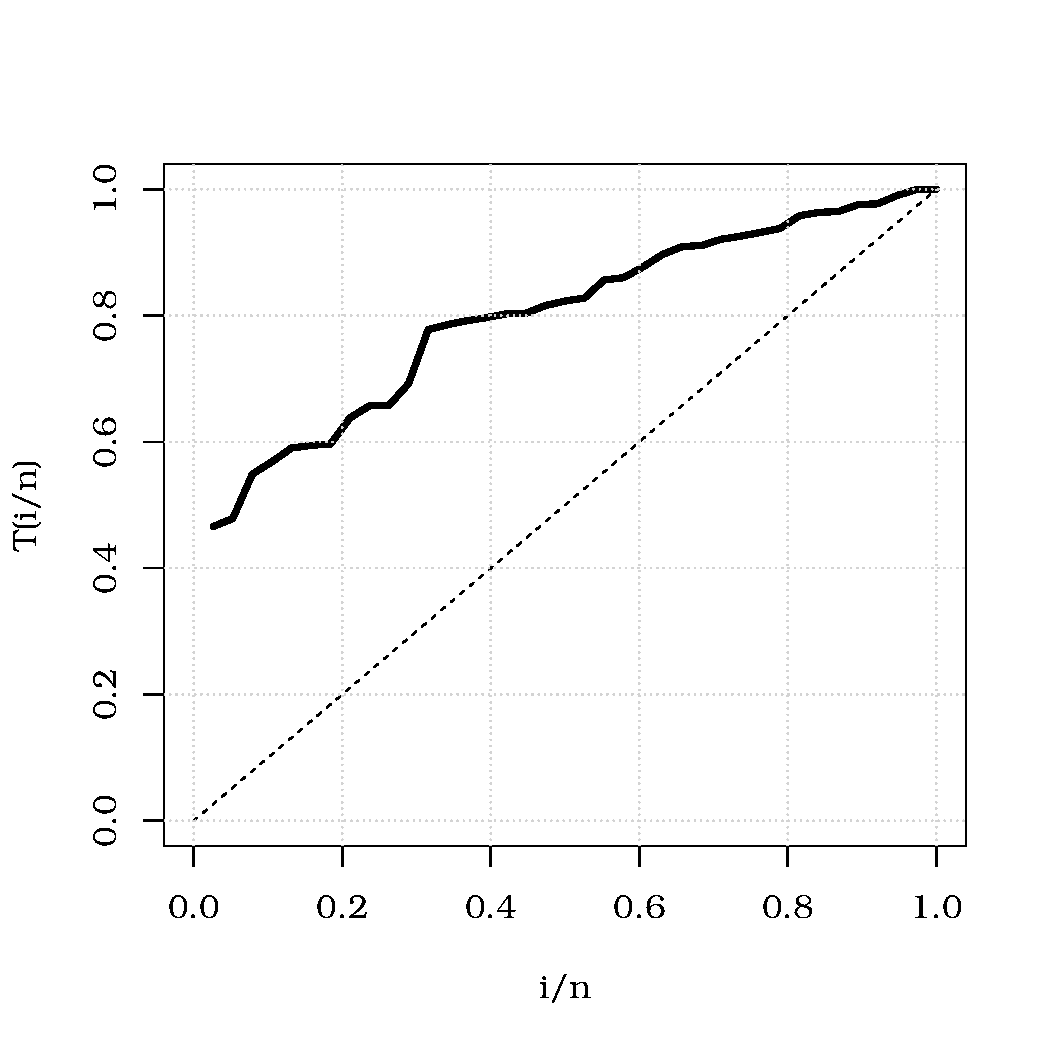
\includegraphics[height=8cm, width=8cm]{TTT_app_1.pdf}
\caption{TTT plot for the food data.\label{ttt}}
\end{center}
\end{figure}


The MLEs, their standard errors (SEs) (in parentheses), and the statistics W$^{*}$ and A$^{*}$ for the fitted models to the current data are listed in Table \ref{tab-ex1}. The results indicate that the proposed model has better performance than the other seven fitted models.

\begin{table}[H]
\scriptsize
\center
\caption{\small Estimation results for food data.}
\label{tab-ex1}
\scalebox{1.1}{
\begin{tabular}{lcccccc}
\hline\noalign{\smallskip}
Model & $\hat{a}$ & $\hat{\theta}$ & $\hat{\lambda}$ & $\hat{\gamma}$ &  $W^*$ & $A^*$   \\
\hline \\
 & & & & &  \\
MOGa-W$(a,\theta,\lambda,\gamma)$    &  0.9261 & 1.3796 & 33.3230 & 25.3988 & 0.0339 &  0.2376 \\                            &    (0.0262) & (0.2238) & (0.2853) & (0.0825)  & & \\

 & & & & &  \\
$\beta-$W$(a,\theta,\lambda,\gamma)$ &   9.9288 &  0.1700 & 9.7594 & 1.5305  & 0.0435 & 0.2594\\
&    (0.0290) & (0.0204) & ($<$0.0001) & ($<$0.0001)  && \\
                                                                                & & & & &  \\
KW-W$(a,\theta,\lambda,\gamma)$ &    0.0498 & 99.9998 &  1.0760 & 23.4028 & 1.3309 & 6.7426\\
 &    (0.0080) & (16.2259) &  (0.0031) &  (0.0146) && \\																						 & & & & &  \\
MOE-W$(a,\theta,\lambda,\gamma)$  &  0.1366 & 2.0204 & 62.7220 & 4.2956  &0.0354 & 0.2579 \\
 & (0.1599) & ($<$0.0001) &($<$0.0001) & (0.7365)    &  & \\
                                                                              & & & & &  \\
EGW$(a,b,\lambda,\gamma)$    &  5.6189 &  6.1833 &  1.2870  & 1.3798  &  0.0371 & 0.2518 \\
& (0.0028) & (0.0009) & (0.1159) & (0.1480)    &  & \\
                                                           & & & & &  \\
MO-W$(a,\lambda,\gamma)$  & 0.1592  & - &  1.5860  & 4.2671  &  0.0345   & 0.2573\\
&    (0.0717) & (-) & (0.1335) & (0.1665)  &  & \\

 & & & & &  \\
exp-W$(a,\lambda,\gamma)$   &    6.1102   & - &   4.4680 &  1.3858 &   0.0372   & 0.2523 \\
&   (0.4222) & (-) & (0.3175) & (0.1677)   &  & \\

 & & & & &  \\
$\gamma$-W$(a,\lambda,\gamma)$    & 5.7515  & - &  10.0000 & 1.2087&  0.0879 & 0.6599  \\
&  (0.0015)&  (-)&  (0.0001) &(0.0082)    &  & \\

 & & & & &  \\
\hline
\end{tabular}}
\end{table}

A data set collected in a pilot study about hypertension in the Dominican Republic in 1997 refers to the second application. The observations are the systolic blood pressure of persons who came to medical clinics in several villages for a variety of complaints. The observations for the data set in question are:
         150,
         120,
         120,
         180,
         138,
         115,
         130,
         150,
         200,
         120,
         190,
         90,
         130,
         120,
         200,
         140,
         110,
         134,
         160,
         140,
         105,
         126,
         129,
         120,
         100,
         130,
         118,
         144,
         180,
         138,
         110,
         140,
         120,
         118,
         110,
         110,
         130,
         140,
         130,
         165,
         180,
         130,
         140,
         112,
         130,
         158,
         112,
         150,
         140,
         142,
         110,
         140,
         130,
         132,
         140,
         140,
         122,
         128,
         90,
         118,
         120,
         110,
         122,
         200,
         110,
         140,
         150,
         120,
         150,
         120,
         164,
         122,
         112,
         130,
         140,
         102,
         122,
         130,
         102,
         130,
         122,
         200,
         140,
         180,
         124,
         110,
         124,
         90,
         120,
         159,
         142,
         140,
         118,
         122,
         108,
         170,
         120,
         140,
         100,
         118,
         110,
         114,
         150,
         160,
         140,
         190,
         118,
         120,
         150,
         120,
         200,
         150,
         168,
         110,
         142,
         150,
         160,
         142,
         160,
         150,
         110,
         128,
         122,
         150,
         140,
         122,
         120,
         130,
         100,
         130,
         150,
         130,
         100,
         120,
         105,
         100,
         150,
         196,
         130,
         110,
         140,
         122,
         110,
         164,
         120,
         120,
         150,
         160,
         150,
         135,
         124,
         110,
         100,
         95,
         130,
         120,
         108,
         118,
         170,
         105,
         120,
         95,
         95,
         120,
         140,
         142,
         160,
         110,
         190,
         180,
         130,
         130,
         120,
         204,
         150,
         150,
         120,
         122,
         120,
         130,
         140,
         148,
         118,
         126,
         136,
         140,
         130,
         102,
         110,
         110,
         130,
         126,
         142,
         140,
         128,
         130,
         124,
         162,
         130,
         130,
         110,
         80,
         166,
         140,
         160,
         160,
         140,
         98,
         138,
         120,
         112,
         112,
         134,
         140,
         115,
         140,
         98,
         115,
         120,
         80,
         160,
         126,
         110,
         130,
         104,
         236,
         118,
         120,
         140,
         120,
         98,
         164,
         150,
         110,
         120,
         130,
         170,
         180,
         110,
         120,
         130,
         118,
         130,
         190,
         158,
         90,
         99,
         210,
         180,
         140,
         184,
         105,
         120,
         150,
         140,
         130,
         160,
         118,
         210,
         100,
         170,
         150,
         130,
         170,
         150,
         120,
         134,
         90,
         125,
         170,
         140,
         150,
         110,
         105,
         140,
         120,
         100,
         124,
         112,
         160,
         140,
         118,
         190,
         110,
         118,
         160,
         150,
         124,
         128,
         150,
         120,
         125,
         118,
         132,
         110,
         143,
         170,
         98,
         124,
         180,
         178,
         110,
         98,
         159,
         110,
         140,
         130,
         122,
         110,
         98,
         180,
         90,
         118,
         165,
         138,
         138,
         170,
         106,
         170,
         140,
         90,
         118,
         110,
         102,
         102,
         180,
         100,
         110,
         162,
         140,
         110,
         98,
         140,
         140,
         110,
         170,
         112,
         90,
         102,
         106,
         124,
         110,
         180,
         138,
         90,
         150,
         126,
         110,
         130,
         150,
         145,
         140,
         156,
         110,
         150,
         160,
         120,
         140,
         120,
         110,
         120,
         140,
         160,
         160,
         110,
         150,
         118,
         110,
         120,
         120,
         146,
         124,
         170,
         124,
         170,
         159,
         120,
         120,
         118,
         152,
         190.



Table \ref{tabds2} provides the descriptive statistics for the second data set. Consi\-dering that the systolic blood pressure represents the highest number presented in the pressure measuring equipment, the maximum (236) found in this 
table should represent an individual with serious heart problems. This is due to the fact that the normal systolic pressure is 120.
 
The minimum value (80) should be for an individual who probably suffers from low blood pressure. Also note that the data set has positive skewness. This indicates that few people have high pressure values and, in this case, the mode is 120, which represents a good value for systolic pressure.

Figure \ref{ttt2} provides the TTT plot for the second clinic data, which shows that the hazard function is decreasing, thus supporting the MOGa-W model.

\begin{figure}[H]
\begin{center}
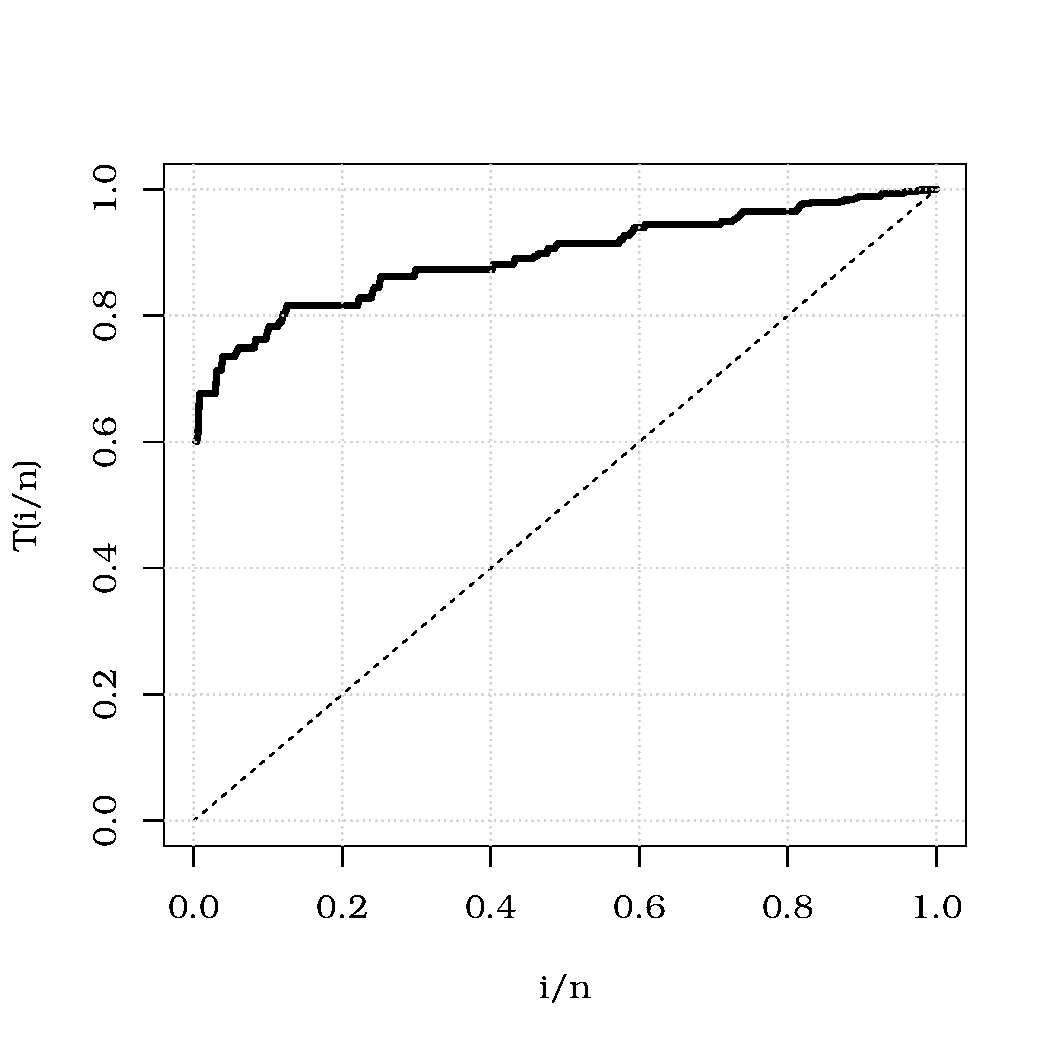
\includegraphics[height=8cm, width=8cm]{TTT_app_2.pdf}
\caption{TTT plot for the clinic data.\label{ttt2}}
\end{center}
\end{figure}

\begin{table}[H] 
%\scriptsize
\center
\caption{Descriptive statistics for the clinic data.}
\label{tabds2}
\begin{tabular}{lr}
\hline\noalign{\smallskip}
   Minimum & 80\\
   1st Qu.& 118\\
   Median&  130\\
   Mean& 133 \\
   3rd  Qu.&  150 \\
   Maximum &  236\\
   Standard Deviation & 25.7157\\
   Skewness & 0.7893\\
   Kurtosis & 0.5908\\
\hline
\end{tabular}
\end{table}

The MLEs of the parameters, their SEs and the values of the adequacy measures for the fitted models to the clinic data 
are reported in Table \ref{tab-ex2}. By comparing the measure values, the proposed distribution outperforms all other 
fitted models. 

\begin{table}[H]
\scriptsize
\center
\caption{\small Estimation results for clinic data.}
\label{tab-ex2}
\scalebox{1.1}{
\begin{tabular}{lcccccc}
\hline\noalign{\smallskip}
Model & $\hat{a}$ & $\hat{\theta}$ & $\hat{\lambda}$ & $\hat{\gamma}$ &  $W^*$ & $A^*$   \\
\hline
 & & & & &  \\
MOGa-W$(a,\theta,\lambda,\gamma)$    &  9.6293 & 3.6407 & 6.2608 & 12.8234 &0.5093&  2.8076 \\
                                       &    (0.0062) & (0.1824) & (0.0244) & (0.0079)  && \\

 & & & & &  \\
 $\beta-$W$(a,\theta,\lambda,\gamma)$ &   31.0847 &  47.1463 &   0.0169 &  2.0540 & 0.7540 & 4.2794\\
&    (0.0127) & ($<$0.0001) & (0.0001) & ($<$0.0001)  && \\

 & & & & &  \\
KW-W$(a,\theta,\lambda,\gamma)$ &   7363.2810 & 0.0392 &  1.4676 &   0.6146 & 0.5351 & 2.9617\\
&    (0.0419) & (0.0004)& ($<$0.0001)& ($<$0.0001) && \\

 & & & & &  \\
 MOE-W$(a,\theta,\lambda,\gamma)$  &  101.1347 &  0.4238  & 0.0309 &  1.7024  &1.1441 & 6.6446 \\
 & (46.7828) &  (0.1008) &  (0.0036) &  (0.1681)   &  & \\

 & & & & &  \\
 EGW$(a,b,\lambda,\gamma)$    &  0.2351&  140.0000 &   0.4576 &   0.7425 &  0.8925 & 5.3338 \\
 & (0.0025) & (3.2785) & ($<$0.0001) & ($<$0.0001)   &  & \\

 & & & & &  \\
 MO-W$(a,\lambda,\gamma)$  & 173.2139  & - &  0.0212 &  1.6019  &  1.4760   & 8.5870\\                                &    (0.0001) & (-) & (0.0002) & (0.0001)  &  & \\

 & & & & &  \\
 exp-W$(a,\lambda,\gamma)$   &    69.0291  & - &   0.0240 & 1.3455 &   0.8899   & 5.0941 \\
                          &   (0.0838) & (-) & (0.0002) & ($<$0.0001)   &  & \\

 & & & & &  \\
 $\Gamma$-W$(a,\lambda,\gamma)$    & 9.1122   & - &  0.0261 & 1.7464 &    0.6227 & 3.4882  \\
                             &  (0.9633)&  (-)&  (0.0029) & (0.0803)     &  & \\

 & & & & &  \\
                          \hline
\end{tabular}}
\end{table}


\section{MATHEMATICAL PROPERTIES}\label{properties}

Here, some mathematical properties for the MOGa-G family are presented based on a linear representation for its density 
function in terms of ``exponentiated-G'' (exp-G) densities.

\subsection{Linear Representation}

For an arbitrary CDF $G(x)$, the CDF and PDF of the exp-G distribution with power parameter $a>0$ are
\begin{eqnarray*}
\Pi_a(x)=G(x)^a\qquad\text{and}\qquad\pi_a(x)=a\,g(x)\,G(x)^{a-1},
\end{eqnarray*}
respectively. This class of distributions is quite useful 
in several applications. In fact, Tahir and Nadarajah (2015)
cited more than seventy papers on exponentiated distributions 
in their Table 1.

First, the CDF of the MO-G distribution (\ref{densityMO}) 
admits the linear representation (Barreto-Souza et al., 2013) \cite{Barreto-Souza}
\begin{equation}
F_{\text{MO}-\Gamma}(x) 
\,=\,
\sum^{\infty}_{i=0}\,w_i^{\text{MO-G}}\,\Pi_{i+1}(x)\,=\,\sum^{\infty}_{i=0}\,w_i^{\text{MO-G}}\,G(x)^{i+1},
\label{EXP44}
\end{equation}
where the coefficients are (for $i=0,1,\ldots$)
\[
w_i^{\text{MO}-\Gamma}=w_i^{\text{MO}-\Gamma}(\theta) =
\begin{cases}
\dfrac{(-1)^i\,\theta}{(i+1)} \sum\limits^{\infty}_{j=i}(j+1)\,\dbinom{j}{i}\,\bar{\theta}^j,& \quad \theta\in (0,1),\\
\theta^{-1} (1-\theta^{-1})^i,& \quad \theta>1,
\end{cases}
\]
and $\bar{\theta}=1-\theta$.

Second, the linear combination for the $\Gamma\text{-G}$ cumulative distribution (\ref{PDF_Ga}) follows from Castellares and Lemonte (2015) \cite{Castellares} as
\begin{equation}\label{EXP33}
F_{\Gamma\text{-G}}(x)\,=\,\sum_{j=0}^\infty w_{j}^{\Gamma\text{-G}}\,\,\Pi_{a+j}(x).
\end{equation}
Here,
$$w_j^{\Gamma\text{-G}}=w_j^{\Gamma\text{-G}}(a)=\frac{\varphi_{j}(a)}{(a+j)},$$
\begin{equation*}\label{coeficientes}
\varphi_0(a)=\frac{1}{\Gamma(a)},
\quad\,
\varphi_j(a)=\frac{(a-1)}{\Gamma(a)}\,\psi_{j-1}(j+a-2),\quad j\geq 1,
\end{equation*}
and
\begin{align*}\label{polinomios_ward}
\begin{split}
\psi_{n-1}(x)&=\frac{(-1)^{n-1}}{(n+1)!}\Biggl[H^{n-1}_{n}-\frac{x+2}{n+2}H^{n-2}_{n}
+ \frac{(x+2)(x+3)}{(n+2)(n+3)}H^{n-3}_{n}- \cdots\\
&\qquad+ (-1)^{n-1}\frac{(x+2)(x+3)\cdots(x+n)}{(n+2)(n+3)\cdots(2n)}H^{0}_{n}\Biggr],
\end{split}
\end{align*}
is the Stirling polynomial, $H^{m}_{n+1}=(2n+1-m)H^{m}_{n} + (n-m+1)H^{m-1}_{n}$ is a positive integer,
$H^0_0=1$, $H^{0}_{n+1}=1\times 3\times 5\times\cdots\times(2n+1)$ and $H^{n}_{n+1}=1$.

By inserting \eqref{EXP33} in Equation \eqref{EXP44} and via a result for a power series raised to a positive integer (Gradshteyn and Ryzhik, 2000) \cite{Gradshteyn}, the expansion for the cdf of the MOGa-G distribution reduces to
\begin{align*}
F_{\text{MO}-\Gamma\text{-G}}(x)&=\sum_{i=0}^{\infty}\,w_{i}^{\text{MO-}\Gamma}\,G(x)^{(i+1)a}\,\left[\sum_{j=0}^{\infty}\,w_{j}^{\Gamma\text{-G}}\,G(x)^{j}\right]^{i+1}\\
&=\sum_{i=0}^{\infty}\,w_{i}^{\text{MO-}\Gamma}\,G(x)^{(i+1)a}\,\sum_{j=0}^{\infty}\,c_{i+1,j}\,G(x)^{j} =\sum_{i,j=0}^\infty d_{i,j}\,\Pi_{(i+1)a+j}(x),
\end{align*}
where $d_{i,j}=d_{i,j}(a,\theta)=w_{i}^{\text{MO-G}}\,c_{i+1,j}(a)$, $c_{i+1,0}(a)=(w_{0}^{\Gamma\text{-G}})^{i+1}$ and, for $m \ge 1$,
$c_{i+1,m}(a)=\frac{1}{m w_{0}^{\Gamma\text{-G}}}\,\sum^{m}_{r=1}\,\left[r(i+2)-m\right]\,w_{r}^{\Gamma\text{-G}}\,c_{i+1,m-r}(a)$.

By differentiating the last equation, the linear representation 
for the MOGa-G density holds
\begin{equation}\label{lcom}
f_{\text{MO}-\Gamma\text{-G}}(x)=\sum_{i,j=0}^\infty d_{i,j}\,\pi_{(i+1)a+j}(x).
\end{equation}

So, some structural properties of the proposed family can be determined from the double linear combination (\ref{lcom})
and those properties of the exp-G distribution. In most applications, the indices $i$ and $j$ can vary up to a small 
number of terms. 


\subsection{Some quantities}

Hereafter, let $T_{i,j}\sim$exp-G$[(i+1)a+j]$. The $n$th moment of $X$ can be determined from (\ref{lcom}) as
{\footnotesize
\begin{eqnarray}\label{moment}
\displaystyle
\mu_n^{\prime}=E(X^n)=\sum_{i,j=0}^\infty d_{i,j}\,E(T_{i,j})=\sum_{i,j=0}^\infty \,[(i+1)a+j-1]\,d_{i,j}\,\tau[n,(i+1)a+j-1],
\end{eqnarray}
}
where
\begin{eqnarray*}
\tau(n,a)=\int_{-\infty}^{\infty} x^n\,G(x)^{a}\,g(x)dx=\int_{0}^{1} Q_G(u)^n\,u^a d u.
\end{eqnarray*}

Expressions for moments of several exponentiated distributions can be found in the papers cited in Tahir and Nadarajah (2015, Table 1). We give just one example from Equation (\ref{moment})
by taking the exponential distribution with rate $\lambda>0$ for the baseline G.
It follows easily as
\begin{eqnarray*}
\mu_n^{\prime}= n!\,\lambda^n\,\sum_{i,j,m=0}^\infty \,\frac{(-1)^{n+m}\,[(i+1)a+j]\,d_{i,j}}{(m+1)^{n+1}}\,\binom{(i+1)a+j-1}{m}.
\end{eqnarray*}

For empirical purposes, the shape of many distributions can be usefully described by the incomplete moments. These moments play an important role for measuring
inequa\-lity. For example, the mean deviations and Lorenz and Bonferroni curves depend upon the first incomplete moment of the distribution.
The $n$th incomplete moment of $X$ can be expressed as
{\footnotesize
\begin{eqnarray}\label{incomplete}
\displaystyle
\qquad
m_{n}(y)=\int_{-\infty}^y x^n\,f_{X}(x) dx = \sum_{i,j=0}^{\infty} [(i+1)a+j]\,d_{i,j}\,\int_{0}^{G(y)}\,Q_G(u)^n\, u^{(i+1)a+j-1}\,du.
\end{eqnarray}
}
The definite integral in (\ref{incomplete}) can be evaluated for most baseline G distributions.

The moment generating function (MGF) $M(t)=E(\rm{e}^{t\,X})$ of $X$ can be expressed from (\ref{lcom})
{\footnotesize
\begin{eqnarray}\label{mgf}
\displaystyle
M(t)=\sum_{i,j=0}^{\infty} \,d_{i,j}\,M_{i,j}(t)=\sum_{i,j=0}^{\infty}\, [(i+1)a+j]\,d_{i,j}\,\rho(t,(i+1)a+j-1),
\end{eqnarray}
}
where $M_{i,j}(t)$ is the MGF of $Y_{i,j}$ and
\begin{eqnarray*}
\rho(t,a)=\int_{-\infty}^{\infty}\,\rm{e}^{t x}\,G(x)^{a}\,g(x) dx=\int_{0}^{1}\exp\left\{t\,Q_G(u)\right\}\,u^a d u.
\end{eqnarray*}

The MGFs of several MOGa-G distributions can be determined from Equation (\ref{mgf}). For example, the generating function of the MOGa-exponential with parameter $\lambda$
(if $t<\lambda^{-1}$) is
\begin{eqnarray*}
\displaystyle
M(t)=\sum_{i,j=0}^{\infty} [(i+1)a+j]\,d_{i,j}\,\,B((i+1)a+j,1-\lambda t).
\end{eqnarray*}


\section{CONCLUSIONS}\label{conclusions}

A new family of distributions called the Marshall and Olkin-Gamma-G family with two shape parameters is introduced. The estimation of the unknown parameters is done via the maximum likelihood method and a simulation study is conducted to verify its adequacy. Additionally, the usefulness of the proposed family is shown empirically by means of two applications to real data. In fact, the new family can generate very competitive distributions with the same number of parameters than others constructed by existing classes.


\begin{thebibliography}{8}

\bibitem{Tahir} Tahir, M. H., Nadarajah, S. (2015).  Parameter induction in continuous univariate distributions: Well-established G families. \textit{Anais da Academia Brasileira de Ciências}, {\bf 87}, 539--568.

\bibitem{Eugene} Eugene, N., Lee, C.,  Famoye, F. (2002). Beta-normal distribution and its applications. \textit{Communications in Statistics-Theory and methods}, {\bf 31}, 4, 497--512.

\bibitem{Zografos} Zografos, K., Balakrishnan, N. (2009). On families of beta-and generalized gamma-generated distributions and associated inference. \textit{Statistical methodology}, {\bf 6}, 4, 344--362.

\bibitem{Marshall} Marshall, A. W.,  Olkin, I. (1997).  A new method for adding a parameter to a family of distributions with application to the exponential and Weibull families. \textit{Biometrika}, {\bf 84}, 3, 641--652.

\bibitem{Marinho} Marinho, P. R. D., Silva, R. B., Bourguignon, M., Cordeiro, G. M.,  Nadarajah, S. (2019). AdequacyModel: An R package for probability distributions and general purpose optimization. \textit{PloS one}, {\bf 14}, 8, e0221487.

\bibitem{Team} Team, R. C. (2022). R: A language and environment for statistical computing. \textit{R Foundation for Statistical Computing}, Vienna, Austria. \url{http://www. R-project. org/}.

\bibitem{Rizzo} Rizzo, Maria L. (2019). Statistical computing with R. \textit{CRC Press}.

\bibitem{Famoye} Famoye, F., Lee, C., Olumolade, O. (2005). The beta-Weibull distribution. \textit{Journal of Statistical Theory and Applications}, {\bf 4}, 2, 121--136.

\bibitem{Cordeiro_2010} Cordeiro, G. M., Ortega, E. M., Nadarajah, S. (2010). The Kumaraswamy Weibull distribution with application to failure data. \textit{Journal of the Franklin Institute}, {\bf 347}, 8, 1399--1429.

\bibitem{Ahmad} Ahmad, H. H., Bdair, O. M., Ahsanullah, M.,  Ahsanullah, M. (2017). On Marshall-Olkin Extended Weibull Distribution. \textit{J. Stat. Theory Appl.}, {\bf 16}, 1, 1--17.

\bibitem{Cordeiro_2019} Cordeiro, G. M., Prataviera, F., do Carmo S Lima, M., Ortega, E. M. (2019). The Marshall-Olkin extended flexible Weibull regression model for censored lifetime data. \textit{Model Assisted Statistics and Applications}, {\bf 14}, 1, 1--17.

\bibitem{Mudholkar} Mudholkar, G. S., Srivastava, D. K. (1993). Exponentiated Weibull family for analyzing bathtub failure-rate data. \textit{IEEE transactions on reliability}, {\bf 42}, 2, 299--302.

\bibitem{Cordeiro_2016} Cordeiro, G. M., Maria do Carmo, S. L., Gomes, A. E., da-Silva, C. Q.,  Ortega, E. M. (2016). The gamma extended Weibull distribution. \textit{Journal of Statistical Distributions and Applications}, {\bf 3}, 1, 1--19.

\bibitem{Oguntunde} Oguntunde, P. E., Odetunmibi, O. A., Adejumo, A. O. (2015). On the exponentiated generalized Weibull distribution: A generalization of the Weibull distribution. \textit{Indian Journal of Science and Technology}, {\bf 8}, 35, 1--7.

\bibitem{Belisle} Bélisle, C. J. (1992). Convergence theorems for a class of simulated annealing algorithms on Rd. \textit{Journal of Applied Probability}, {\bf 29}, 4, 885--895.

\bibitem{Barreto-Souza} Barreto-Souza, W., Lemonte, A. J.,  Cordeiro, G. M. (2013). General results for the Marshall and Olkin's family of distributions. \textit{Anais da Academia Brasileira de Ciências}, {\bf 85}, 1, 3--21.

\bibitem{Castellares} Castellares, F., Lemonte, A. J. (2015). A new generalized Weibull distribution generated by gamma random variables. \textit{Journal of the Egyptian Mathematical Society}, {\bf 23}, 2, 382--390.

\bibitem{Gradshteyn} Gradshteyn, I. S.,  Ryzhik, I. M. (2014). Table of integrals, series, and products. \textit{Academic press}.
\end{thebibliography}


\end{document}
